% Apparatus
% • Pump system that can be configured as a single pump or as two pumps in series or
% parallel operation.
% Mec E 403 2
% Centrifugal Pumps
% • Stop watch
% • Strobotach
% • Pressure transducers

% Measurements of pump pressure differential vs. flow rate are required for various operating
% speeds. The manufacturer’s specifications are given in the attached performance curves. The
% impeller has a diameter of 108 mm as shown in Figure 3.
% The pump pressure differential is measured using a calibrated pressure transducer connected
% to pressure taps located upstream of the pump suction inlet and downstream from the outlet.
% Mec E 403 8
% Centrifugal Pumps
% Figure 5: Two pumps operating in parallel
% The suction line has a diameter of 50.8 mm and the discharge line has a diameter of 38.1 mm.
% The flow rate is determined by diverting the flow to a weighing tank and using a stopwatch
% to collect a known quantity of water.
% 1. One pump should be tested individually at 3 speeds specified by the teaching assistant,
% ranging from one-half to full speed. The speed of the pump will be determined using
% the strobotach.
% 2. At each pump speed, the flow rates at 4 different pressures should be recorded (shutoff,
% full open and two other equally spaced intermediate settings). Make sure to adjust the
% speed of the pump to the correct value when changing the pressures before taking any
% other readings. At each operating condition you should record
% a) pump speed (make sure it is set to the correct value),
% b) pressure transducer output,
% c) the moment arm and dyno mass (to determine the torque produced by the motor)
% d) time required to collect a known quantity of water.
% 3. This procedure will then be repeated for parallel and series system configurations with
% both pumps set at full speed (or as specified by the teaching assistant).

\section{Procedure}
\begin{figure}[h]
    \centering
    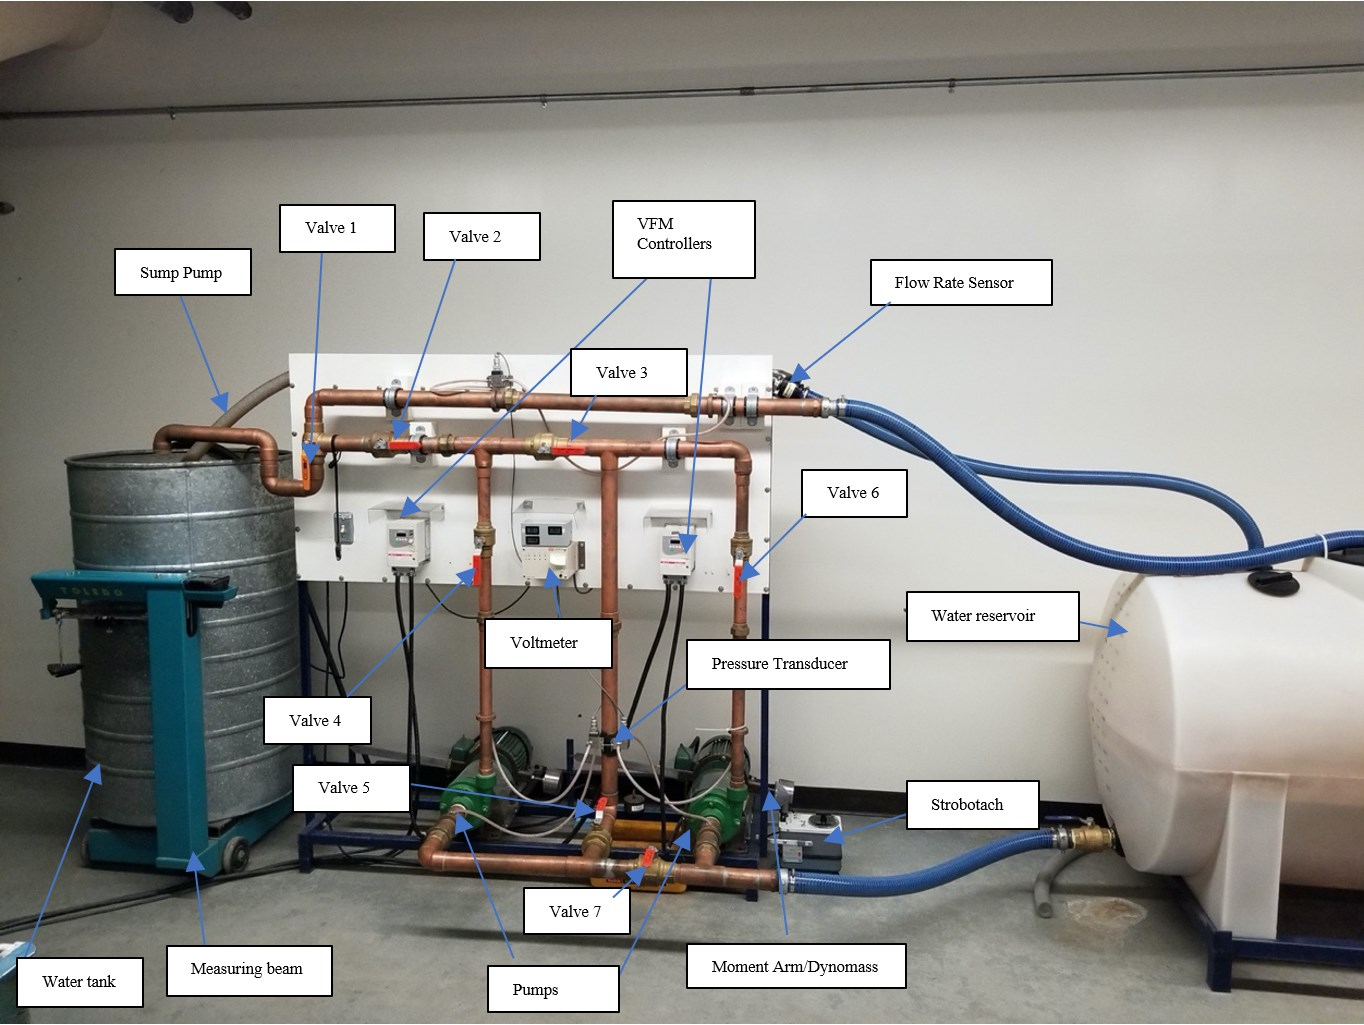
\includegraphics[width=0.5\textwidth]{Sections/Figures/Experimental Setup.jpg}
    \caption{Experimental setup for the pump system}
\end{figure}
\subsection{Equipment}
\begin{itemize}
    \item Pump system that can be configured as a single pump or as two pumps in series or parallel operation. This is the system being studied.
    \item Stopwatch to measure time to fill a container 
    \item Strobotach to verify pump rotational speed
    \item Mass scale to measure 200 lbs of water
    \item 1.401 kg mass to measure moment arm (torque) of motor
    \item Pressure transducers to measure pump pressure differential
\end{itemize}

\subsection{Procedure}
\begin{enumerate}[label=\arabic*.]
    \item The pump system will be tested in single pump configuration at 1800, 2700, and 3600 RPM. The speed of the pump will be verified using the strobotach.
    \item At each pump speed, the following measurements at four different pressures will be recorded (shutoff, full open, and two other equally spaced intermediate settings):
    \begin{enumerate}[label=\roman*.]
        \item Time to fill a container to $\qty{200}{lbs}$ of water will be recorded three times.
        \item Pressure transducer(s) voltage output will be recorded.
        \item The moment arm and dyno mass will be recorded to determine the torque produced by the motor.
    \end{enumerate}
    Make sure to clear the water container after recording a time with the sump pump. A total of 36 time measurements will be recorded for the single pump configuration.
    \item Item (2) will be repeated for parallel and series system configurations with both pumps set at 2700 RPM (neglect the 1800 and 3600 RPM configurations for parallel and series systems). Neglect recording the moment arm and ensure the output of both pressure transducers are recorded. A total of 24 time measurements will be recorded for the parallel and series configurations.
\end{enumerate} 